\batchmode
\documentclass[twoside]{book}

% Packages required by doxygen
\usepackage{calc}
\usepackage{doxygen}
\usepackage{graphicx}
\usepackage[utf8]{inputenc}
\usepackage{makeidx}
\usepackage{multicol}
\usepackage{multirow}
\usepackage{fixltx2e}
\PassOptionsToPackage{warn}{textcomp}
\usepackage{textcomp}
\usepackage[nointegrals]{wasysym}
\usepackage[table]{xcolor}

% Font selection
\usepackage[T1]{fontenc}
\usepackage{mathptmx}
\usepackage[scaled=.90]{helvet}
\usepackage{courier}
\usepackage{amssymb}
\usepackage{sectsty}
\renewcommand{\familydefault}{\sfdefault}
\allsectionsfont{%
  \fontseries{bc}\selectfont%
  \color{darkgray}%
}
\renewcommand{\DoxyLabelFont}{%
  \fontseries{bc}\selectfont%
  \color{darkgray}%
}
\newcommand{\+}{\discretionary{\mbox{\scriptsize$\hookleftarrow$}}{}{}}

% Page & text layout
\usepackage{geometry}
\geometry{%
  a4paper,%
  top=2.5cm,%
  bottom=2.5cm,%
  left=2.5cm,%
  right=2.5cm%
}
\tolerance=750
\hfuzz=15pt
\hbadness=750
\setlength{\emergencystretch}{15pt}
\setlength{\parindent}{0cm}
\setlength{\parskip}{0.2cm}
\makeatletter
\renewcommand{\paragraph}{%
  \@startsection{paragraph}{4}{0ex}{-1.0ex}{1.0ex}{%
    \normalfont\normalsize\bfseries\SS@parafont%
  }%
}
\renewcommand{\subparagraph}{%
  \@startsection{subparagraph}{5}{0ex}{-1.0ex}{1.0ex}{%
    \normalfont\normalsize\bfseries\SS@subparafont%
  }%
}
\makeatother

% Headers & footers
\usepackage{fancyhdr}
\pagestyle{fancyplain}
\fancyhead[LE]{\fancyplain{}{\bfseries\thepage}}
\fancyhead[CE]{\fancyplain{}{}}
\fancyhead[RE]{\fancyplain{}{\bfseries\leftmark}}
\fancyhead[LO]{\fancyplain{}{\bfseries\rightmark}}
\fancyhead[CO]{\fancyplain{}{}}
\fancyhead[RO]{\fancyplain{}{\bfseries\thepage}}
\fancyfoot[LE]{\fancyplain{}{}}
\fancyfoot[CE]{\fancyplain{}{}}
\fancyfoot[RE]{\fancyplain{}{\bfseries\scriptsize Generated on Sun Jun 22 2014 21\+:13\+:20 for epeg by Doxygen }}
\fancyfoot[LO]{\fancyplain{}{\bfseries\scriptsize Generated on Sun Jun 22 2014 21\+:13\+:20 for epeg by Doxygen }}
\fancyfoot[CO]{\fancyplain{}{}}
\fancyfoot[RO]{\fancyplain{}{}}
\renewcommand{\footrulewidth}{0.4pt}
\renewcommand{\chaptermark}[1]{%
  \markboth{#1}{}%
}
\renewcommand{\sectionmark}[1]{%
  \markright{\thesection\ #1}%
}

% Indices & bibliography
\usepackage{natbib}
\usepackage[titles]{tocloft}
\setcounter{tocdepth}{3}
\setcounter{secnumdepth}{5}
\makeindex

% Hyperlinks (required, but should be loaded last)
\usepackage{ifpdf}
\ifpdf
  \usepackage[pdftex,pagebackref=true]{hyperref}
\else
  \usepackage[ps2pdf,pagebackref=true]{hyperref}
\fi
\hypersetup{%
  colorlinks=true,%
  linkcolor=blue,%
  citecolor=blue,%
  unicode%
}

% Custom commands
\newcommand{\clearemptydoublepage}{%
  \newpage{\pagestyle{empty}\cleardoublepage}%
}


%===== C O N T E N T S =====

\begin{document}

% Titlepage & ToC
\hypersetup{pageanchor=false,
             bookmarks=true,
             bookmarksnumbered=true,
             pdfencoding=unicode
            }
\pagenumbering{roman}
\begin{titlepage}
\vspace*{7cm}
\begin{center}%
{\Large epeg \\[1ex]\large 0.\+9.\+0 }\\
\vspace*{1cm}
{\large Generated by Doxygen 1.8.7}\\
\vspace*{0.5cm}
{\small Sun Jun 22 2014 21:13:20}\\
\end{center}
\end{titlepage}
\clearemptydoublepage
\tableofcontents
\clearemptydoublepage
\pagenumbering{arabic}
\hypersetup{pageanchor=true}

%--- Begin generated contents ---
\chapter{Epeg Library Documentation}
\label{index}\hypertarget{index}{} \begin{DoxyVersion}{Version}
0.\+9.\+0 
\end{DoxyVersion}
\begin{DoxyAuthor}{Author}
Carsten Haitzler \href{mailto:raster@rasterman.com}{\texttt{ raster@rasterman.\+com}} 
\end{DoxyAuthor}
\begin{DoxyDate}{Date}
2000-\/2003
\end{DoxyDate}
\hypertarget{index_intro}{}\doxysection{What is Epeg?}\label{index_intro}
An IMMENSELY FAST JPEG thumbnailer library API.

Why write this? It is a convenience library API to using libjpeg to load JPEG images destined to be turned into thumbnails of the original, saving information with these thumbnails, retreiving it and managing to load the image ready for scaling with the minimum of fuss and CPU overhead.

This means that it is insanely fast at loading large JPEG images and scaling them down to tiny thumbnails. The speedup that it provides will be proportional to the size difference between the source image and the output thumbnail size as a count of their pixels.

It makes use of libjpeg features of being able to load an image by only decoding the DCT coefficients needed to reconstruct an image of the size desired. This gives a massive speedup. If you do NOT try to access the pixels in a format other than YUV (or GRAY8 if the source is grascale), then it also avoids colorspace conversions as well.

Using the library is very easy; look at this example\+:


\begin{DoxyCode}{0}
\DoxyCodeLine{\textcolor{preprocessor}{\#include <stdio.h>} \textcolor{comment}{/* for printf() */}}
\DoxyCodeLine{\textcolor{preprocessor}{\#include <stdlib.h>} \textcolor{comment}{/* for exit() */}}
\DoxyCodeLine{\textcolor{preprocessor}{\#include "{}Epeg.h"{}}}
\DoxyCodeLine{}
\DoxyCodeLine{\textcolor{keywordtype}{int} main(\textcolor{keywordtype}{int} argc, \textcolor{keywordtype}{char} **argv)}
\DoxyCodeLine{\{}
\DoxyCodeLine{   Epeg\_Image *im;}
\DoxyCodeLine{}
\DoxyCodeLine{   \textcolor{keywordflow}{if} (argc != 3) \{}
\DoxyCodeLine{        printf(\textcolor{stringliteral}{"{}Usage: \%s input.jpg thumb.jpg\(\backslash\)n"{}}, argv[0]);}
\DoxyCodeLine{        exit(0);}
\DoxyCodeLine{   \}}
\DoxyCodeLine{   im = \mbox{\hyperlink{epeg_8c_a8295f48501747f18cbb74e4eb1c55836}{epeg\_file\_open}}(argv[1]);}
\DoxyCodeLine{   \textcolor{keywordflow}{if} (!im) \{}
\DoxyCodeLine{        printf(\textcolor{stringliteral}{"{}Cannot open \%s\(\backslash\)n"{}}, argv[1]);}
\DoxyCodeLine{        exit(-\/1);}
\DoxyCodeLine{   \}}
\DoxyCodeLine{   }
\DoxyCodeLine{   \mbox{\hyperlink{epeg_8c_a800dc04316740427b1f4366d973ff4e4}{epeg\_decode\_size\_set}}(im, 128, 96);}
\DoxyCodeLine{   \mbox{\hyperlink{epeg_8c_ad0c11f61561f622ca4097c47c75129bc}{epeg\_quality\_set}}(im, 75);}
\DoxyCodeLine{   \mbox{\hyperlink{epeg_8c_a5cfe689f77dbe7b120317a195585ee51}{epeg\_thumbnail\_comments\_enable}}(im, 1);}
\DoxyCodeLine{   \mbox{\hyperlink{epeg_8c_a4aa4c7bbf3edf1f24603d3b4dad684b4}{epeg\_file\_output\_set}}(im, argv[2]);}
\DoxyCodeLine{   \mbox{\hyperlink{epeg_8c_a12a018084510ebdc0e627f56305fea79}{epeg\_encode}}(im);}
\DoxyCodeLine{   \mbox{\hyperlink{epeg_8c_a8faf0f0fab47ac97b86ee7e00e1bee7c}{epeg\_close}}(im);}
\DoxyCodeLine{   }
\DoxyCodeLine{   \textcolor{keywordflow}{return} 0;}
\DoxyCodeLine{\}}

\end{DoxyCode}


This program exists as epeg\+\_\+test.\+c so that you can compile this program with as small a line as\+:

\begin{DoxyVerb}gcc epeg_test.c -o epeg_test `epeg-config --cflags --libs`
\end{DoxyVerb}


It is a very simple library that just makes life easier when trying to generate lots of thumbnails for large JPEG images as quickly as possible. Your milage may vary, but it should save you lots of time and effort in using libjpeg in general.

\begin{DoxyRefDesc}{Todo}
\item[\mbox{\hyperlink{todo__todo000001}{Todo}}]Check all input parameters for sanity. 

Actually report error conditions properly.\end{DoxyRefDesc}

\chapter{Todo List}
\label{todo}
\hypertarget{todo}{}

\begin{DoxyRefList}
\item[\label{todo__todo000001}%
\hypertarget{todo__todo000001}{}%
page \hyperlink{index}{Epeg Library Documentation} ]Check all input parameters for sanity. 

Actually report error conditions properly.
\end{DoxyRefList}
\chapter{File Index}
\section{File List}
Here is a list of all documented files with brief descriptions\-:\begin{DoxyCompactList}
\item\contentsline{section}{\hyperlink{epeg_8c}{epeg.\-c} \\*Epeg J\-P\-E\-G Thumbnailer library }{\pageref{epeg_8c}}{}
\end{DoxyCompactList}

\chapter{File Documentation}
\hypertarget{epeg_8c}{\section{epeg.\+c File Reference}
\label{epeg_8c}\index{epeg.\+c@{epeg.\+c}}
}


Epeg J\+P\+E\+G Thumbnailer library.  


{\ttfamily \#include $<$stdio.\+h$>$}\\*
{\ttfamily \#include $<$stdlib.\+h$>$}\\*
{\ttfamily \#include \char`\"{}Epeg.\+h\char`\"{}}\\*
{\ttfamily \#include \char`\"{}epeg\+\_\+private.\+h\char`\"{}}\\*
Include dependency graph for epeg.\+c\+:
\nopagebreak
\begin{figure}[H]
\begin{center}
\leavevmode
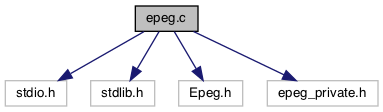
\includegraphics[width=350pt]{epeg_8c__incl}
\end{center}
\end{figure}
\subsection*{Functions}
\begin{DoxyCompactItemize}
\item 
Epeg\+\_\+\+Image $\ast$ \hyperlink{epeg_8c_a8295f48501747f18cbb74e4eb1c55836}{epeg\+\_\+file\+\_\+open} (const char $\ast$file)
\begin{DoxyCompactList}\small\item\em Open a J\+P\+E\+G image by filename. \end{DoxyCompactList}\item 
Epeg\+\_\+\+Image $\ast$ \hyperlink{epeg_8c_a55d449402ab7ad9de9febd63b858a2dc}{epeg\+\_\+memory\+\_\+open} (unsigned char $\ast$data, int size)
\begin{DoxyCompactList}\small\item\em Open a J\+P\+E\+G image stored in memory. \end{DoxyCompactList}\item 
void \hyperlink{epeg_8c_a3b8680bdbf470d1a634618e5308ce147}{epeg\+\_\+size\+\_\+get} (Epeg\+\_\+\+Image $\ast$im, int $\ast$w, int $\ast$h)
\begin{DoxyCompactList}\small\item\em Return the original J\+P\+E\+G pixel size. \end{DoxyCompactList}\item 
void \hyperlink{epeg_8c_a290a722dddc53761d213524ce0e89284}{epeg\+\_\+colorspace\+\_\+get} (Epeg\+\_\+\+Image $\ast$im, int $\ast$space)
\begin{DoxyCompactList}\small\item\em Return the original J\+P\+E\+G pixel color space. \end{DoxyCompactList}\item 
void \hyperlink{epeg_8c_a800dc04316740427b1f4366d973ff4e4}{epeg\+\_\+decode\+\_\+size\+\_\+set} (Epeg\+\_\+\+Image $\ast$im, int w, int h)
\begin{DoxyCompactList}\small\item\em Set the size of the image to decode in pixels. \end{DoxyCompactList}\item 
void \hyperlink{epeg_8c_ab840f7b7ea8c21938a5210dee06e9dda}{epeg\+\_\+decode\+\_\+bounds\+\_\+set} (Epeg\+\_\+\+Image $\ast$im, int x, int y, int w, int h)
\begin{DoxyCompactList}\small\item\em Set the bounds of the image to decode in pixels. \end{DoxyCompactList}\item 
void \hyperlink{epeg_8c_afe41e06c6667542ad4685730538e03f7}{epeg\+\_\+decode\+\_\+colorspace\+\_\+set} (Epeg\+\_\+\+Image $\ast$im, Epeg\+\_\+\+Colorspace colorspace)
\begin{DoxyCompactList}\small\item\em Set the colorspace in which to decode the image. \end{DoxyCompactList}\item 
const void $\ast$ \hyperlink{epeg_8c_acf990fda661066b46bbf470830288c78}{epeg\+\_\+pixels\+\_\+get} (Epeg\+\_\+\+Image $\ast$im, int x, int y, int w, int h)
\begin{DoxyCompactList}\small\item\em Get a segment of decoded pixels from an image. \end{DoxyCompactList}\item 
const void $\ast$ \hyperlink{epeg_8c_ac1d79775e08f47098507ac265581bf63}{epeg\+\_\+pixels\+\_\+get\+\_\+as\+\_\+\+R\+G\+B8} (Epeg\+\_\+\+Image $\ast$im, int x, int y, int w, int h)
\begin{DoxyCompactList}\small\item\em Get a segment of decoded pixels from an image. \end{DoxyCompactList}\item 
void \hyperlink{epeg_8c_adf9efc5d877afebda99aba8d5c2bbb0f}{epeg\+\_\+pixels\+\_\+free} (Epeg\+\_\+\+Image $\ast$im, const void $\ast$data)
\begin{DoxyCompactList}\small\item\em Free requested pixel block from an image. \end{DoxyCompactList}\item 
const char $\ast$ \hyperlink{epeg_8c_acf6013949f1cf3b4b5fc7f086fdaabaa}{epeg\+\_\+comment\+\_\+get} (Epeg\+\_\+\+Image $\ast$im)
\begin{DoxyCompactList}\small\item\em Get the image comment field as a string. \end{DoxyCompactList}\item 
void \hyperlink{epeg_8c_a28e230b7b3bb05b8a470c80c45100c52}{epeg\+\_\+thumbnail\+\_\+comments\+\_\+get} (Epeg\+\_\+\+Image $\ast$im, Epeg\+\_\+\+Thumbnail\+\_\+\+Info $\ast$info)
\begin{DoxyCompactList}\small\item\em Get thumbnail comments of loaded image. \end{DoxyCompactList}\item 
void \hyperlink{epeg_8c_ab96605b1c21ec8d791df705a5117233c}{epeg\+\_\+comment\+\_\+set} (Epeg\+\_\+\+Image $\ast$im, const char $\ast$comment)
\begin{DoxyCompactList}\small\item\em Set the comment field of the image for saving. \end{DoxyCompactList}\item 
void \hyperlink{epeg_8c_ad0c11f61561f622ca4097c47c75129bc}{epeg\+\_\+quality\+\_\+set} (Epeg\+\_\+\+Image $\ast$im, int quality)
\begin{DoxyCompactList}\small\item\em Set the encoding quality of the saved image. \end{DoxyCompactList}\item 
void \hyperlink{epeg_8c_a5cfe689f77dbe7b120317a195585ee51}{epeg\+\_\+thumbnail\+\_\+comments\+\_\+enable} (Epeg\+\_\+\+Image $\ast$im, int onoff)
\begin{DoxyCompactList}\small\item\em Enable thumbnail comments in saved image. \end{DoxyCompactList}\item 
void \hyperlink{epeg_8c_a4aa4c7bbf3edf1f24603d3b4dad684b4}{epeg\+\_\+file\+\_\+output\+\_\+set} (Epeg\+\_\+\+Image $\ast$im, const char $\ast$file)
\begin{DoxyCompactList}\small\item\em Set the output file path for the image when saved. \end{DoxyCompactList}\item 
void \hyperlink{epeg_8c_ae0e91c160074e6d96b7e366fb0eb6ec8}{epeg\+\_\+memory\+\_\+output\+\_\+set} (Epeg\+\_\+\+Image $\ast$im, unsigned char $\ast$$\ast$data, int $\ast$size)
\begin{DoxyCompactList}\small\item\em Set the output file to be a block of allocated memory. \end{DoxyCompactList}\item 
int \hyperlink{epeg_8c_a12a018084510ebdc0e627f56305fea79}{epeg\+\_\+encode} (Epeg\+\_\+\+Image $\ast$im)
\begin{DoxyCompactList}\small\item\em This saves the image to its specified destination. \end{DoxyCompactList}\item 
int \hyperlink{epeg_8c_a327dab144744ba5f1892643d627e6df0}{epeg\+\_\+trim} (Epeg\+\_\+\+Image $\ast$im)
\begin{DoxyCompactList}\small\item\em F\+I\+X\+M\+E\+: Document this with a short, sentence-\/long description of \hyperlink{epeg_8c_a327dab144744ba5f1892643d627e6df0}{epeg\+\_\+trim()} \end{DoxyCompactList}\item 
void \hyperlink{epeg_8c_a8faf0f0fab47ac97b86ee7e00e1bee7c}{epeg\+\_\+close} (Epeg\+\_\+\+Image $\ast$im)
\begin{DoxyCompactList}\small\item\em Close an image handle. \end{DoxyCompactList}\end{DoxyCompactItemize}


\subsection{Detailed Description}
Epeg J\+P\+E\+G Thumbnailer library. 

These routines are used for the Epeg library. 

\subsection{Function Documentation}
\hypertarget{epeg_8c_a8faf0f0fab47ac97b86ee7e00e1bee7c}{\index{epeg.\+c@{epeg.\+c}!epeg\+\_\+close@{epeg\+\_\+close}}
\index{epeg\+\_\+close@{epeg\+\_\+close}!epeg.\+c@{epeg.\+c}}
\subsubsection[{epeg\+\_\+close}]{\setlength{\rightskip}{0pt plus 5cm}void epeg\+\_\+close (
\begin{DoxyParamCaption}
\item[{Epeg\+\_\+\+Image $\ast$}]{im}
\end{DoxyParamCaption}
)}}\label{epeg_8c_a8faf0f0fab47ac97b86ee7e00e1bee7c}


Close an image handle. 


\begin{DoxyParams}{Parameters}
{\em im} & A handle to an opened Epeg image. \\
\hline
\end{DoxyParams}
\begin{DoxyReturn}{Returns}
Nothing.
\end{DoxyReturn}
This closes an opened image handle and frees all memory associated with it. It does N\+O\+T free encoded data generated by \hyperlink{epeg_8c_ae0e91c160074e6d96b7e366fb0eb6ec8}{epeg\+\_\+memory\+\_\+output\+\_\+set()} followed by \hyperlink{epeg_8c_a12a018084510ebdc0e627f56305fea79}{epeg\+\_\+encode()}, nor does it guarantee to free any data received by \hyperlink{epeg_8c_acf990fda661066b46bbf470830288c78}{epeg\+\_\+pixels\+\_\+get()}. Once an image handle is closed, consider it invalid.

See also\+: \hyperlink{epeg_8c_a8295f48501747f18cbb74e4eb1c55836}{epeg\+\_\+file\+\_\+open()}, \hyperlink{epeg_8c_a55d449402ab7ad9de9febd63b858a2dc}{epeg\+\_\+memory\+\_\+open()} 

Referenced by epeg\+\_\+file\+\_\+open(), and epeg\+\_\+memory\+\_\+open().



Here is the caller graph for this function\+:
\nopagebreak
\begin{figure}[H]
\begin{center}
\leavevmode
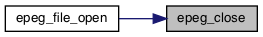
\includegraphics[width=292pt]{epeg_8c_a8faf0f0fab47ac97b86ee7e00e1bee7c_icgraph}
\end{center}
\end{figure}


\hypertarget{epeg_8c_a290a722dddc53761d213524ce0e89284}{\index{epeg.\+c@{epeg.\+c}!epeg\+\_\+colorspace\+\_\+get@{epeg\+\_\+colorspace\+\_\+get}}
\index{epeg\+\_\+colorspace\+\_\+get@{epeg\+\_\+colorspace\+\_\+get}!epeg.\+c@{epeg.\+c}}
\subsubsection[{epeg\+\_\+colorspace\+\_\+get}]{\setlength{\rightskip}{0pt plus 5cm}void epeg\+\_\+colorspace\+\_\+get (
\begin{DoxyParamCaption}
\item[{Epeg\+\_\+\+Image $\ast$}]{im, }
\item[{int $\ast$}]{space}
\end{DoxyParamCaption}
)}}\label{epeg_8c_a290a722dddc53761d213524ce0e89284}


Return the original J\+P\+E\+G pixel color space. 


\begin{DoxyParams}{Parameters}
{\em im} & A handle to an opened Epeg image. \\
\hline
{\em space} & A pointer to the color space value to be filled in. \\
\hline
\end{DoxyParams}
\begin{DoxyReturn}{Returns}
Nothing.
\end{DoxyReturn}
Returns the image color space (not yet though).

See also\+: \hyperlink{epeg_8c_a3b8680bdbf470d1a634618e5308ce147}{epeg\+\_\+size\+\_\+get()} \hypertarget{epeg_8c_acf6013949f1cf3b4b5fc7f086fdaabaa}{\index{epeg.\+c@{epeg.\+c}!epeg\+\_\+comment\+\_\+get@{epeg\+\_\+comment\+\_\+get}}
\index{epeg\+\_\+comment\+\_\+get@{epeg\+\_\+comment\+\_\+get}!epeg.\+c@{epeg.\+c}}
\subsubsection[{epeg\+\_\+comment\+\_\+get}]{\setlength{\rightskip}{0pt plus 5cm}const char $\ast$ epeg\+\_\+comment\+\_\+get (
\begin{DoxyParamCaption}
\item[{Epeg\+\_\+\+Image $\ast$}]{im}
\end{DoxyParamCaption}
)}}\label{epeg_8c_acf6013949f1cf3b4b5fc7f086fdaabaa}


Get the image comment field as a string. 


\begin{DoxyParams}{Parameters}
{\em im} & A handle to an opened Epeg image. \\
\hline
\end{DoxyParams}
\begin{DoxyReturn}{Returns}
A pointer to the loaded image comments.
\end{DoxyReturn}
This function returns the comment field as a string (N\+U\+L byte terminated) of the loaded image {\ttfamily im}, if there is a comment, or N\+U\+L\+L if no comment is saved with the image. Consider the string returned to be read-\/only.

See also\+: \hyperlink{epeg_8c_a28e230b7b3bb05b8a470c80c45100c52}{epeg\+\_\+thumbnail\+\_\+comments\+\_\+get()} \hypertarget{epeg_8c_ab96605b1c21ec8d791df705a5117233c}{\index{epeg.\+c@{epeg.\+c}!epeg\+\_\+comment\+\_\+set@{epeg\+\_\+comment\+\_\+set}}
\index{epeg\+\_\+comment\+\_\+set@{epeg\+\_\+comment\+\_\+set}!epeg.\+c@{epeg.\+c}}
\subsubsection[{epeg\+\_\+comment\+\_\+set}]{\setlength{\rightskip}{0pt plus 5cm}void epeg\+\_\+comment\+\_\+set (
\begin{DoxyParamCaption}
\item[{Epeg\+\_\+\+Image $\ast$}]{im, }
\item[{const char $\ast$}]{comment}
\end{DoxyParamCaption}
)}}\label{epeg_8c_ab96605b1c21ec8d791df705a5117233c}


Set the comment field of the image for saving. 


\begin{DoxyParams}{Parameters}
{\em im} & A handle to an opened Epeg image. \\
\hline
{\em comment} & The comment to set. \\
\hline
\end{DoxyParams}
\begin{DoxyReturn}{Returns}
Nothing.
\end{DoxyReturn}
Set the comment for the image file for when it gets saved. This is a N\+U\+L byte terminated C string. If {\ttfamily comment} is N\+U\+L\+L the output file will have no comment field.

The default comment will be any comment loaded from the input file.

See also\+: \hyperlink{epeg_8c_acf6013949f1cf3b4b5fc7f086fdaabaa}{epeg\+\_\+comment\+\_\+get()} \hypertarget{epeg_8c_ab840f7b7ea8c21938a5210dee06e9dda}{\index{epeg.\+c@{epeg.\+c}!epeg\+\_\+decode\+\_\+bounds\+\_\+set@{epeg\+\_\+decode\+\_\+bounds\+\_\+set}}
\index{epeg\+\_\+decode\+\_\+bounds\+\_\+set@{epeg\+\_\+decode\+\_\+bounds\+\_\+set}!epeg.\+c@{epeg.\+c}}
\subsubsection[{epeg\+\_\+decode\+\_\+bounds\+\_\+set}]{\setlength{\rightskip}{0pt plus 5cm}void epeg\+\_\+decode\+\_\+bounds\+\_\+set (
\begin{DoxyParamCaption}
\item[{Epeg\+\_\+\+Image $\ast$}]{im, }
\item[{int}]{x, }
\item[{int}]{y, }
\item[{int}]{w, }
\item[{int}]{h}
\end{DoxyParamCaption}
)}}\label{epeg_8c_ab840f7b7ea8c21938a5210dee06e9dda}


Set the bounds of the image to decode in pixels. 


\begin{DoxyParams}{Parameters}
{\em im} & A handle to an opened Epeg image. \\
\hline
{\em x} & Boundary X \\
\hline
{\em y} & Boundary Y \\
\hline
{\em w} & Boundary W \\
\hline
{\em h} & Boundary H \\
\hline
\end{DoxyParams}
\begin{DoxyReturn}{Returns}
Nothing.
\end{DoxyReturn}
Sets the bounds inside which to decode the J\+P\+E\+G image, giving an optimized load that only decodes the bounded pixels. (???)

See also\+: \hyperlink{epeg_8c_a800dc04316740427b1f4366d973ff4e4}{epeg\+\_\+decode\+\_\+size\+\_\+set()}, \hyperlink{epeg_8c_afe41e06c6667542ad4685730538e03f7}{epeg\+\_\+decode\+\_\+colorspace\+\_\+set()} \hypertarget{epeg_8c_afe41e06c6667542ad4685730538e03f7}{\index{epeg.\+c@{epeg.\+c}!epeg\+\_\+decode\+\_\+colorspace\+\_\+set@{epeg\+\_\+decode\+\_\+colorspace\+\_\+set}}
\index{epeg\+\_\+decode\+\_\+colorspace\+\_\+set@{epeg\+\_\+decode\+\_\+colorspace\+\_\+set}!epeg.\+c@{epeg.\+c}}
\subsubsection[{epeg\+\_\+decode\+\_\+colorspace\+\_\+set}]{\setlength{\rightskip}{0pt plus 5cm}void epeg\+\_\+decode\+\_\+colorspace\+\_\+set (
\begin{DoxyParamCaption}
\item[{Epeg\+\_\+\+Image $\ast$}]{im, }
\item[{Epeg\+\_\+\+Colorspace}]{colorspace}
\end{DoxyParamCaption}
)}}\label{epeg_8c_afe41e06c6667542ad4685730538e03f7}


Set the colorspace in which to decode the image. 


\begin{DoxyParams}{Parameters}
{\em im} & A handle to an opened Epeg image. \\
\hline
{\em colorspace} & The colorspace to decode the image in. \\
\hline
\end{DoxyParams}
\begin{DoxyReturn}{Returns}
Nothing.
\end{DoxyReturn}
This sets the colorspace to decode the image in. The default is E\+P\+E\+G\+\_\+\+Y\+U\+V8, as this is normally the native colorspace of a J\+P\+E\+G file, avoiding any colorspace conversions for a faster load and/or save.

See also\+: \hyperlink{epeg_8c_a800dc04316740427b1f4366d973ff4e4}{epeg\+\_\+decode\+\_\+size\+\_\+set()}, \hyperlink{epeg_8c_ab840f7b7ea8c21938a5210dee06e9dda}{epeg\+\_\+decode\+\_\+bounds\+\_\+set()} \hypertarget{epeg_8c_a800dc04316740427b1f4366d973ff4e4}{\index{epeg.\+c@{epeg.\+c}!epeg\+\_\+decode\+\_\+size\+\_\+set@{epeg\+\_\+decode\+\_\+size\+\_\+set}}
\index{epeg\+\_\+decode\+\_\+size\+\_\+set@{epeg\+\_\+decode\+\_\+size\+\_\+set}!epeg.\+c@{epeg.\+c}}
\subsubsection[{epeg\+\_\+decode\+\_\+size\+\_\+set}]{\setlength{\rightskip}{0pt plus 5cm}void epeg\+\_\+decode\+\_\+size\+\_\+set (
\begin{DoxyParamCaption}
\item[{Epeg\+\_\+\+Image $\ast$}]{im, }
\item[{int}]{w, }
\item[{int}]{h}
\end{DoxyParamCaption}
)}}\label{epeg_8c_a800dc04316740427b1f4366d973ff4e4}


Set the size of the image to decode in pixels. 


\begin{DoxyParams}{Parameters}
{\em im} & A handle to an opened Epeg image. \\
\hline
{\em w} & The width of the image to decode at, in pixels. \\
\hline
{\em h} & The height of the image to decode at, in pixels. \\
\hline
\end{DoxyParams}
\begin{DoxyReturn}{Returns}
Nothing.
\end{DoxyReturn}
Sets the size at which to decode the J\+P\+E\+G image, giving an optimized load that only decodes the pixels needed.

See also\+: \hyperlink{epeg_8c_ab840f7b7ea8c21938a5210dee06e9dda}{epeg\+\_\+decode\+\_\+bounds\+\_\+set()}, \hyperlink{epeg_8c_afe41e06c6667542ad4685730538e03f7}{epeg\+\_\+decode\+\_\+colorspace\+\_\+set()} \hypertarget{epeg_8c_a12a018084510ebdc0e627f56305fea79}{\index{epeg.\+c@{epeg.\+c}!epeg\+\_\+encode@{epeg\+\_\+encode}}
\index{epeg\+\_\+encode@{epeg\+\_\+encode}!epeg.\+c@{epeg.\+c}}
\subsubsection[{epeg\+\_\+encode}]{\setlength{\rightskip}{0pt plus 5cm}int epeg\+\_\+encode (
\begin{DoxyParamCaption}
\item[{Epeg\+\_\+\+Image $\ast$}]{im}
\end{DoxyParamCaption}
)}}\label{epeg_8c_a12a018084510ebdc0e627f56305fea79}


This saves the image to its specified destination. 


\begin{DoxyParams}{Parameters}
{\em im} & A handle to an opened Epeg image. \\
\hline
\end{DoxyParams}
\begin{DoxyReturn}{Returns}
1 if something happened, otherwise 0.
\end{DoxyReturn}
This saves the image {\ttfamily im} to its destination specified by \hyperlink{epeg_8c_a4aa4c7bbf3edf1f24603d3b4dad684b4}{epeg\+\_\+file\+\_\+output\+\_\+set()} or \hyperlink{epeg_8c_ae0e91c160074e6d96b7e366fb0eb6ec8}{epeg\+\_\+memory\+\_\+output\+\_\+set()}. The image will be encoded at the decoded pixel size, using the quality, comment, and thumbnail comment settings set on the image.

See also\+: \hyperlink{epeg_8c_a4aa4c7bbf3edf1f24603d3b4dad684b4}{epeg\+\_\+file\+\_\+output\+\_\+set()}, \hyperlink{epeg_8c_ae0e91c160074e6d96b7e366fb0eb6ec8}{epeg\+\_\+memory\+\_\+output\+\_\+set()} \hypertarget{epeg_8c_a8295f48501747f18cbb74e4eb1c55836}{\index{epeg.\+c@{epeg.\+c}!epeg\+\_\+file\+\_\+open@{epeg\+\_\+file\+\_\+open}}
\index{epeg\+\_\+file\+\_\+open@{epeg\+\_\+file\+\_\+open}!epeg.\+c@{epeg.\+c}}
\subsubsection[{epeg\+\_\+file\+\_\+open}]{\setlength{\rightskip}{0pt plus 5cm}Epeg\+\_\+\+Image $\ast$ epeg\+\_\+file\+\_\+open (
\begin{DoxyParamCaption}
\item[{const char $\ast$}]{file}
\end{DoxyParamCaption}
)}}\label{epeg_8c_a8295f48501747f18cbb74e4eb1c55836}


Open a J\+P\+E\+G image by filename. 


\begin{DoxyParams}{Parameters}
{\em file} & The file path to open. \\
\hline
\end{DoxyParams}
\begin{DoxyReturn}{Returns}
A handle to the opened J\+P\+E\+G file, with the header decoded.
\end{DoxyReturn}
This function opens the file indicated by the {\ttfamily file} parameter, and attempts to decode it as a jpeg file. If this failes, N\+U\+L\+L is returned. Otherwise a valid handle to an open J\+P\+E\+G file is returned that can be used by other Epeg calls.

The {\ttfamily file} must be a pointer to a valid C string, N\+U\+L (0 byte) terminated thats is a relative or absolute file path. If not results are not determined.

See also\+: \hyperlink{epeg_8c_a55d449402ab7ad9de9febd63b858a2dc}{epeg\+\_\+memory\+\_\+open()}, \hyperlink{epeg_8c_a8faf0f0fab47ac97b86ee7e00e1bee7c}{epeg\+\_\+close()} 

References epeg\+\_\+close().



Here is the call graph for this function\+:
\nopagebreak
\begin{figure}[H]
\begin{center}
\leavevmode
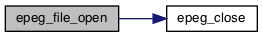
\includegraphics[width=269pt]{epeg_8c_a8295f48501747f18cbb74e4eb1c55836_cgraph}
\end{center}
\end{figure}


\hypertarget{epeg_8c_a4aa4c7bbf3edf1f24603d3b4dad684b4}{\index{epeg.\+c@{epeg.\+c}!epeg\+\_\+file\+\_\+output\+\_\+set@{epeg\+\_\+file\+\_\+output\+\_\+set}}
\index{epeg\+\_\+file\+\_\+output\+\_\+set@{epeg\+\_\+file\+\_\+output\+\_\+set}!epeg.\+c@{epeg.\+c}}
\subsubsection[{epeg\+\_\+file\+\_\+output\+\_\+set}]{\setlength{\rightskip}{0pt plus 5cm}void epeg\+\_\+file\+\_\+output\+\_\+set (
\begin{DoxyParamCaption}
\item[{Epeg\+\_\+\+Image $\ast$}]{im, }
\item[{const char $\ast$}]{file}
\end{DoxyParamCaption}
)}}\label{epeg_8c_a4aa4c7bbf3edf1f24603d3b4dad684b4}


Set the output file path for the image when saved. 


\begin{DoxyParams}{Parameters}
{\em im} & A handle to an opened Epeg image. \\
\hline
{\em file} & The path to the output file. \\
\hline
\end{DoxyParams}
\begin{DoxyReturn}{Returns}
Nothing.
\end{DoxyReturn}
This sets the output file path name (either a full or relative path name) to where the file will be written when saved. {\ttfamily file} must be a N\+U\+L terminated C string containing the path to the file to be saved to. If it is N\+U\+L\+L, then the image will not be saved to a file when calling \hyperlink{epeg_8c_a12a018084510ebdc0e627f56305fea79}{epeg\+\_\+encode()}.

See also\+: \hyperlink{epeg_8c_ae0e91c160074e6d96b7e366fb0eb6ec8}{epeg\+\_\+memory\+\_\+output\+\_\+set()}, \hyperlink{epeg_8c_a12a018084510ebdc0e627f56305fea79}{epeg\+\_\+encode()} \hypertarget{epeg_8c_a55d449402ab7ad9de9febd63b858a2dc}{\index{epeg.\+c@{epeg.\+c}!epeg\+\_\+memory\+\_\+open@{epeg\+\_\+memory\+\_\+open}}
\index{epeg\+\_\+memory\+\_\+open@{epeg\+\_\+memory\+\_\+open}!epeg.\+c@{epeg.\+c}}
\subsubsection[{epeg\+\_\+memory\+\_\+open}]{\setlength{\rightskip}{0pt plus 5cm}Epeg\+\_\+\+Image $\ast$ epeg\+\_\+memory\+\_\+open (
\begin{DoxyParamCaption}
\item[{unsigned char $\ast$}]{data, }
\item[{int}]{size}
\end{DoxyParamCaption}
)}}\label{epeg_8c_a55d449402ab7ad9de9febd63b858a2dc}


Open a J\+P\+E\+G image stored in memory. 


\begin{DoxyParams}{Parameters}
{\em data} & A pointer to the memory containing the J\+P\+E\+G data. \\
\hline
{\em size} & The size of the memory segment containing the J\+P\+E\+G. \\
\hline
\end{DoxyParams}
\begin{DoxyReturn}{Returns}
A handle to the opened J\+P\+E\+G, with the header decoded.
\end{DoxyReturn}
This function opens a J\+P\+E\+G file that is stored in memory pointed to by {\ttfamily data}, and that is {\ttfamily size} bytes in size. If successful a valid handle is returned, or on failure N\+U\+L\+L is returned.

See also\+: \hyperlink{epeg_8c_a8295f48501747f18cbb74e4eb1c55836}{epeg\+\_\+file\+\_\+open()}, \hyperlink{epeg_8c_a8faf0f0fab47ac97b86ee7e00e1bee7c}{epeg\+\_\+close()} 

References epeg\+\_\+close().



Here is the call graph for this function\+:
\nopagebreak
\begin{figure}[H]
\begin{center}
\leavevmode
\includegraphics[width=292pt]{epeg_8c_a55d449402ab7ad9de9febd63b858a2dc_cgraph}
\end{center}
\end{figure}


\hypertarget{epeg_8c_ae0e91c160074e6d96b7e366fb0eb6ec8}{\index{epeg.\+c@{epeg.\+c}!epeg\+\_\+memory\+\_\+output\+\_\+set@{epeg\+\_\+memory\+\_\+output\+\_\+set}}
\index{epeg\+\_\+memory\+\_\+output\+\_\+set@{epeg\+\_\+memory\+\_\+output\+\_\+set}!epeg.\+c@{epeg.\+c}}
\subsubsection[{epeg\+\_\+memory\+\_\+output\+\_\+set}]{\setlength{\rightskip}{0pt plus 5cm}void epeg\+\_\+memory\+\_\+output\+\_\+set (
\begin{DoxyParamCaption}
\item[{Epeg\+\_\+\+Image $\ast$}]{im, }
\item[{unsigned char $\ast$$\ast$}]{data, }
\item[{int $\ast$}]{size}
\end{DoxyParamCaption}
)}}\label{epeg_8c_ae0e91c160074e6d96b7e366fb0eb6ec8}


Set the output file to be a block of allocated memory. 


\begin{DoxyParams}{Parameters}
{\em im} & A handle to an opened Epeg image. \\
\hline
{\em data} & A pointer to a pointer to a memory block. \\
\hline
{\em size} & A pointer to a counter of the size of the memory block. \\
\hline
\end{DoxyParams}
\begin{DoxyReturn}{Returns}
Nothing.
\end{DoxyReturn}
This sets the output encoding of the image when saved to be allocated memory. After \hyperlink{epeg_8c_a8faf0f0fab47ac97b86ee7e00e1bee7c}{epeg\+\_\+close()} is called the pointer pointed to by {\ttfamily data} and the integer pointed to by {\ttfamily size} will contain the pointer to the memory block and its size in bytes, respecitvely. The memory block can be freed with the free() function call. If the save fails the pointer to the memory block will be unaffected, as will the size.

See also\+: \hyperlink{epeg_8c_a4aa4c7bbf3edf1f24603d3b4dad684b4}{epeg\+\_\+file\+\_\+output\+\_\+set()}, \hyperlink{epeg_8c_a12a018084510ebdc0e627f56305fea79}{epeg\+\_\+encode()} \hypertarget{epeg_8c_adf9efc5d877afebda99aba8d5c2bbb0f}{\index{epeg.\+c@{epeg.\+c}!epeg\+\_\+pixels\+\_\+free@{epeg\+\_\+pixels\+\_\+free}}
\index{epeg\+\_\+pixels\+\_\+free@{epeg\+\_\+pixels\+\_\+free}!epeg.\+c@{epeg.\+c}}
\subsubsection[{epeg\+\_\+pixels\+\_\+free}]{\setlength{\rightskip}{0pt plus 5cm}void epeg\+\_\+pixels\+\_\+free (
\begin{DoxyParamCaption}
\item[{Epeg\+\_\+\+Image $\ast$}]{im, }
\item[{const void $\ast$}]{data}
\end{DoxyParamCaption}
)}}\label{epeg_8c_adf9efc5d877afebda99aba8d5c2bbb0f}


Free requested pixel block from an image. 


\begin{DoxyParams}{Parameters}
{\em im} & A handle to an opened Epeg image (unused). \\
\hline
{\em data} & The pointer to the image pixels. \\
\hline
\end{DoxyParams}
\begin{DoxyReturn}{Returns}
Nothing.
\end{DoxyReturn}
This frees the data for a block of pixels requested from image {\ttfamily im}. {\ttfamily data} must be a valid (non N\+U\+L\+L) pointer to a pixel block taken from the image {\ttfamily im} by \hyperlink{epeg_8c_acf990fda661066b46bbf470830288c78}{epeg\+\_\+pixels\+\_\+get()} and must be called before the image is closed by \hyperlink{epeg_8c_a8faf0f0fab47ac97b86ee7e00e1bee7c}{epeg\+\_\+close()}. \hypertarget{epeg_8c_acf990fda661066b46bbf470830288c78}{\index{epeg.\+c@{epeg.\+c}!epeg\+\_\+pixels\+\_\+get@{epeg\+\_\+pixels\+\_\+get}}
\index{epeg\+\_\+pixels\+\_\+get@{epeg\+\_\+pixels\+\_\+get}!epeg.\+c@{epeg.\+c}}
\subsubsection[{epeg\+\_\+pixels\+\_\+get}]{\setlength{\rightskip}{0pt plus 5cm}const void $\ast$ epeg\+\_\+pixels\+\_\+get (
\begin{DoxyParamCaption}
\item[{Epeg\+\_\+\+Image $\ast$}]{im, }
\item[{int}]{x, }
\item[{int}]{y, }
\item[{int}]{w, }
\item[{int}]{h}
\end{DoxyParamCaption}
)}}\label{epeg_8c_acf990fda661066b46bbf470830288c78}


Get a segment of decoded pixels from an image. 


\begin{DoxyParams}{Parameters}
{\em im} & A handle to an opened Epeg image. \\
\hline
{\em x} & Rectangle X. \\
\hline
{\em y} & Rectangle Y. \\
\hline
{\em w} & Rectangle width. \\
\hline
{\em h} & Rectangle height. \\
\hline
\end{DoxyParams}
\begin{DoxyReturn}{Returns}
Pointer to the top left of the requested pixel block.
\end{DoxyReturn}
Return image pixels in the decoded format from the specified location rectangle bounded with the box {\ttfamily x}, {\ttfamily y} {\ttfamily w} X {\ttfamily y}. The pixel block is packed with no row padding, and it organized from top-\/left to bottom right, row by row. You must free the pixel block using \hyperlink{epeg_8c_adf9efc5d877afebda99aba8d5c2bbb0f}{epeg\+\_\+pixels\+\_\+free()} before you close the image handle, and assume the pixels to be read-\/only memory.

On success the pointer is returned, on failure, N\+U\+L\+L is returned. Failure may be because the rectangle is out of the bounds of the image, memory allocations failed, or the image data cannot be decoded.

See also\+: \hyperlink{epeg_8c_ac1d79775e08f47098507ac265581bf63}{epeg\+\_\+pixels\+\_\+get\+\_\+as\+\_\+\+R\+G\+B8()} \hypertarget{epeg_8c_ac1d79775e08f47098507ac265581bf63}{\index{epeg.\+c@{epeg.\+c}!epeg\+\_\+pixels\+\_\+get\+\_\+as\+\_\+\+R\+G\+B8@{epeg\+\_\+pixels\+\_\+get\+\_\+as\+\_\+\+R\+G\+B8}}
\index{epeg\+\_\+pixels\+\_\+get\+\_\+as\+\_\+\+R\+G\+B8@{epeg\+\_\+pixels\+\_\+get\+\_\+as\+\_\+\+R\+G\+B8}!epeg.\+c@{epeg.\+c}}
\subsubsection[{epeg\+\_\+pixels\+\_\+get\+\_\+as\+\_\+\+R\+G\+B8}]{\setlength{\rightskip}{0pt plus 5cm}const void $\ast$ epeg\+\_\+pixels\+\_\+get\+\_\+as\+\_\+\+R\+G\+B8 (
\begin{DoxyParamCaption}
\item[{Epeg\+\_\+\+Image $\ast$}]{im, }
\item[{int}]{x, }
\item[{int}]{y, }
\item[{int}]{w, }
\item[{int}]{h}
\end{DoxyParamCaption}
)}}\label{epeg_8c_ac1d79775e08f47098507ac265581bf63}


Get a segment of decoded pixels from an image. 


\begin{DoxyParams}{Parameters}
{\em im} & A handle to an opened Epeg image. \\
\hline
{\em x} & Rectangle X. \\
\hline
{\em y} & Rectangle Y. \\
\hline
{\em w} & Rectangle width. \\
\hline
{\em h} & Rectangle height. \\
\hline
\end{DoxyParams}
\begin{DoxyReturn}{Returns}
Pointer to the top left of the requested pixel block.
\end{DoxyReturn}
Return image pixels in the decoded format from the specified location rectangle bounded with the box {\ttfamily x}, {\ttfamily y} {\ttfamily w} X {\ttfamily y}. The pixel block is packed with no row padding, and it organized from top-\/left to bottom right, row by row. You must free the pixel block using \hyperlink{epeg_8c_adf9efc5d877afebda99aba8d5c2bbb0f}{epeg\+\_\+pixels\+\_\+free()} before you close the image handle, and assume the pixels to be read-\/only memory.

On success the pointer is returned, on failure, N\+U\+L\+L is returned. Failure may be because the rectangle is out of the bounds of the image, memory allocations failed, or the image data cannot be decoded.

See also\+: \hyperlink{epeg_8c_acf990fda661066b46bbf470830288c78}{epeg\+\_\+pixels\+\_\+get()} \hypertarget{epeg_8c_ad0c11f61561f622ca4097c47c75129bc}{\index{epeg.\+c@{epeg.\+c}!epeg\+\_\+quality\+\_\+set@{epeg\+\_\+quality\+\_\+set}}
\index{epeg\+\_\+quality\+\_\+set@{epeg\+\_\+quality\+\_\+set}!epeg.\+c@{epeg.\+c}}
\subsubsection[{epeg\+\_\+quality\+\_\+set}]{\setlength{\rightskip}{0pt plus 5cm}void epeg\+\_\+quality\+\_\+set (
\begin{DoxyParamCaption}
\item[{Epeg\+\_\+\+Image $\ast$}]{im, }
\item[{int}]{quality}
\end{DoxyParamCaption}
)}}\label{epeg_8c_ad0c11f61561f622ca4097c47c75129bc}


Set the encoding quality of the saved image. 


\begin{DoxyParams}{Parameters}
{\em im} & A handle to an opened Epeg image. \\
\hline
{\em quality} & The quality of encoding from 0 to 100. \\
\hline
\end{DoxyParams}
\begin{DoxyReturn}{Returns}
Nothing.
\end{DoxyReturn}
Set the quality of the output encoded image. Values from 0 to 100 inclusive are valid, with 100 being the maximum quality, and 0 being the minimum. If the quality is set equal to or above 90\%, the output U and V color planes are encoded at 1\+:1 with the Y plane.

The default quality is 75.

See also\+: \hyperlink{epeg_8c_ab96605b1c21ec8d791df705a5117233c}{epeg\+\_\+comment\+\_\+set()} \hypertarget{epeg_8c_a3b8680bdbf470d1a634618e5308ce147}{\index{epeg.\+c@{epeg.\+c}!epeg\+\_\+size\+\_\+get@{epeg\+\_\+size\+\_\+get}}
\index{epeg\+\_\+size\+\_\+get@{epeg\+\_\+size\+\_\+get}!epeg.\+c@{epeg.\+c}}
\subsubsection[{epeg\+\_\+size\+\_\+get}]{\setlength{\rightskip}{0pt plus 5cm}void epeg\+\_\+size\+\_\+get (
\begin{DoxyParamCaption}
\item[{Epeg\+\_\+\+Image $\ast$}]{im, }
\item[{int $\ast$}]{w, }
\item[{int $\ast$}]{h}
\end{DoxyParamCaption}
)}}\label{epeg_8c_a3b8680bdbf470d1a634618e5308ce147}


Return the original J\+P\+E\+G pixel size. 


\begin{DoxyParams}{Parameters}
{\em im} & A handle to an opened Epeg image. \\
\hline
{\em w} & A pointer to the width value in pixels to be filled in. \\
\hline
{\em h} & A pointer to the height value in pixels to be filled in. \\
\hline
\end{DoxyParams}
\begin{DoxyReturn}{Returns}
Nothing.
\end{DoxyReturn}
Returns the image size in pixels (well not really).

See also\+: \hyperlink{epeg_8c_a290a722dddc53761d213524ce0e89284}{epeg\+\_\+colorspace\+\_\+get()} \hypertarget{epeg_8c_a5cfe689f77dbe7b120317a195585ee51}{\index{epeg.\+c@{epeg.\+c}!epeg\+\_\+thumbnail\+\_\+comments\+\_\+enable@{epeg\+\_\+thumbnail\+\_\+comments\+\_\+enable}}
\index{epeg\+\_\+thumbnail\+\_\+comments\+\_\+enable@{epeg\+\_\+thumbnail\+\_\+comments\+\_\+enable}!epeg.\+c@{epeg.\+c}}
\subsubsection[{epeg\+\_\+thumbnail\+\_\+comments\+\_\+enable}]{\setlength{\rightskip}{0pt plus 5cm}void epeg\+\_\+thumbnail\+\_\+comments\+\_\+enable (
\begin{DoxyParamCaption}
\item[{Epeg\+\_\+\+Image $\ast$}]{im, }
\item[{int}]{onoff}
\end{DoxyParamCaption}
)}}\label{epeg_8c_a5cfe689f77dbe7b120317a195585ee51}


Enable thumbnail comments in saved image. 


\begin{DoxyParams}{Parameters}
{\em im} & A handle to an opened Epeg image. \\
\hline
{\em onoff} & A boolean on and off enabling flag. \\
\hline
\end{DoxyParams}
\begin{DoxyReturn}{Returns}
Nothing.
\end{DoxyReturn}
if {\ttfamily onoff} is 1, the output file will have thumbnail comments added to it, and if it is 0, it will not. The default is 0.

See also\+: \hyperlink{epeg_8c_a28e230b7b3bb05b8a470c80c45100c52}{epeg\+\_\+thumbnail\+\_\+comments\+\_\+get()} \hypertarget{epeg_8c_a28e230b7b3bb05b8a470c80c45100c52}{\index{epeg.\+c@{epeg.\+c}!epeg\+\_\+thumbnail\+\_\+comments\+\_\+get@{epeg\+\_\+thumbnail\+\_\+comments\+\_\+get}}
\index{epeg\+\_\+thumbnail\+\_\+comments\+\_\+get@{epeg\+\_\+thumbnail\+\_\+comments\+\_\+get}!epeg.\+c@{epeg.\+c}}
\subsubsection[{epeg\+\_\+thumbnail\+\_\+comments\+\_\+get}]{\setlength{\rightskip}{0pt plus 5cm}void epeg\+\_\+thumbnail\+\_\+comments\+\_\+get (
\begin{DoxyParamCaption}
\item[{Epeg\+\_\+\+Image $\ast$}]{im, }
\item[{Epeg\+\_\+\+Thumbnail\+\_\+\+Info $\ast$}]{info}
\end{DoxyParamCaption}
)}}\label{epeg_8c_a28e230b7b3bb05b8a470c80c45100c52}


Get thumbnail comments of loaded image. 


\begin{DoxyParams}{Parameters}
{\em im} & A handle to an opened Epeg image. \\
\hline
{\em info} & Pointer to a thumbnail info struct to be filled in. \\
\hline
\end{DoxyParams}
\begin{DoxyReturn}{Returns}
Nothing.
\end{DoxyReturn}
This function retrieves thumbnail comments written by Epeg to any saved J\+P\+E\+G files. If no thumbnail comments were saved, the fields will be 0 in the {\ttfamily info} struct on return.

See also\+: \hyperlink{epeg_8c_acf6013949f1cf3b4b5fc7f086fdaabaa}{epeg\+\_\+comment\+\_\+get()}, \hyperlink{epeg_8c_a5cfe689f77dbe7b120317a195585ee51}{epeg\+\_\+thumbnail\+\_\+comments\+\_\+enable()} \hypertarget{epeg_8c_a327dab144744ba5f1892643d627e6df0}{\index{epeg.\+c@{epeg.\+c}!epeg\+\_\+trim@{epeg\+\_\+trim}}
\index{epeg\+\_\+trim@{epeg\+\_\+trim}!epeg.\+c@{epeg.\+c}}
\subsubsection[{epeg\+\_\+trim}]{\setlength{\rightskip}{0pt plus 5cm}int epeg\+\_\+trim (
\begin{DoxyParamCaption}
\item[{Epeg\+\_\+\+Image $\ast$}]{im}
\end{DoxyParamCaption}
)}}\label{epeg_8c_a327dab144744ba5f1892643d627e6df0}


F\+I\+X\+M\+E\+: Document this with a short, sentence-\/long description of \hyperlink{epeg_8c_a327dab144744ba5f1892643d627e6df0}{epeg\+\_\+trim()} 


\begin{DoxyParams}{Parameters}
{\em im} & A handle to an opened Epeg image. \\
\hline
\end{DoxyParams}
\begin{DoxyReturn}{Returns}
1 if something happened, otherwise 0.
\end{DoxyReturn}
F\+I\+X\+M\+E\+: Document this with a longer, paragraph-\/long description. 
%--- End generated contents ---

% Index
\newpage
\phantomsection
\addcontentsline{toc}{chapter}{Index}
\printindex

\end{document}
